% Chapter Template

\chapter{Nom du chaptitre} % Main chapter title

\label{Chapitre 2} % Change X to a consecutive number; for referencing this chapter elsewhere, use \ref{ChapterX}

\lhead{ \emph{Nom du chaptitre}} % Change X to a consecutive number; this is for the header on each page - perhaps a shortened title

Introduction chapitre

%----------------------------------------------------------------------------------------
%	SECTION 1
%----------------------------------------------------------------------------------------
\section{Nom de la section}

Texte section.
%-----------------------------------
%	SUBSECTION
%-----------------------------------
\subsection{Titre sous section}
Texte sous section
\begin{lstlisting}[frame=single,style=C]  % Start your code-block

int main()
{
	printf("exemple en C\n");
	return 0;
}
\end{lstlisting}


Exemple de texte.

\lstinputlisting[frame=single,style=C, title=main.c]{Ressources/Code_Source/main.c}
%\lstinputlisting[language=Python, firstline=37, lastline=45]{source_filename.py}

Texte
\rem{Ceci est une remarque}

\tmpnew{tmp new: A faire!}


\begin{lstlisting}[frame=single,style=Console]
$ Texte console
\end{lstlisting}
\pagebreak Apès un saut de page.


\begin{center} 
\hspace{12.45cm}
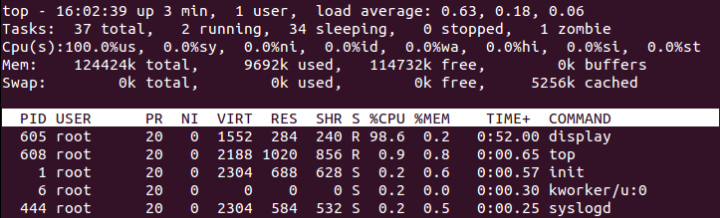
\includegraphics[width=12cm]{image_exemple.png}
\end{center}
\vspace{1cm}

Texte

Liste
\begin{enumerate}
\item Premier
\item Deuxième
\item Dernier
\end{enumerate}


 


